\documentclass[11pt,]{article}
\usepackage[left=1in,top=1in,right=1in,bottom=1in]{geometry}
\newcommand*{\authorfont}{\fontfamily{phv}\selectfont}
\usepackage[]{mathpazo}


  \usepackage[T1]{fontenc}
  \usepackage[utf8]{inputenc}



\usepackage{abstract}
\renewcommand{\abstractname}{}    % clear the title
\renewcommand{\absnamepos}{empty} % originally center

\renewenvironment{abstract}
 {{%
    \setlength{\leftmargin}{0mm}
    \setlength{\rightmargin}{\leftmargin}%
  }%
  \relax}
 {\endlist}

\makeatletter
\def\@maketitle{%
  \newpage
%  \null
%  \vskip 2em%
%  \begin{center}%
  \let \footnote \thanks
    {\fontsize{18}{20}\selectfont\raggedright  \setlength{\parindent}{0pt} \@title \par}%
}
%\fi
\makeatother




\setcounter{secnumdepth}{3}

\usepackage{longtable,booktabs}

\usepackage{graphicx,grffile}
\makeatletter
\def\maxwidth{\ifdim\Gin@nat@width>\linewidth\linewidth\else\Gin@nat@width\fi}
\def\maxheight{\ifdim\Gin@nat@height>\textheight\textheight\else\Gin@nat@height\fi}
\makeatother
% Scale images if necessary, so that they will not overflow the page
% margins by default, and it is still possible to overwrite the defaults
% using explicit options in \includegraphics[width, height, ...]{}
\setkeys{Gin}{width=\maxwidth,height=\maxheight,keepaspectratio}

\title{Asociación y composición florística de la familia Sapotaceae en la
parcela permanente de 50h, Isla Barro Colorado  }



\author{\Large Merali Rosario\vspace{0.05in} \newline\normalsize\emph{Estudiante, Universidad Autónoma de Santo Domingo (UASD)}  }


\date{}

\usepackage{titlesec}

\titleformat*{\section}{\normalsize\bfseries}
\titleformat*{\subsection}{\normalsize\itshape}
\titleformat*{\subsubsection}{\normalsize\itshape}
\titleformat*{\paragraph}{\normalsize\itshape}
\titleformat*{\subparagraph}{\normalsize\itshape}

\titlespacing{\section}
{0pt}{36pt}{0pt}
\titlespacing{\subsection}
{0pt}{36pt}{0pt}
\titlespacing{\subsubsection}
{0pt}{36pt}{0pt}





\newtheorem{hypothesis}{Hypothesis}
\usepackage{setspace}

\makeatletter
\@ifpackageloaded{hyperref}{}{%
\ifxetex
  \PassOptionsToPackage{hyphens}{url}\usepackage[setpagesize=false, % page size defined by xetex
              unicode=false, % unicode breaks when used with xetex
              xetex]{hyperref}
\else
  \PassOptionsToPackage{hyphens}{url}\usepackage[unicode=true]{hyperref}
\fi
}

\@ifpackageloaded{color}{
    \PassOptionsToPackage{usenames,dvipsnames}{color}
}{%
    \usepackage[usenames,dvipsnames]{color}
}
\makeatother
\hypersetup{breaklinks=true,
            bookmarks=true,
            pdfauthor={Merali Rosario (Estudiante, Universidad Autónoma de Santo Domingo (UASD))},
             pdfkeywords = {Diversidad, Sapotaceae, Riqueza, Abundancia, Asociación},  
            pdftitle={Asociación y composición florística de la familia Sapotaceae en la
parcela permanente de 50h, Isla Barro Colorado},
            colorlinks=true,
            citecolor=blue,
            urlcolor=blue,
            linkcolor=magenta,
            pdfborder={0 0 0}}
\urlstyle{same}  % don't use monospace font for urls

% set default figure placement to htbp
\makeatletter
\def\fps@figure{htbp}
\makeatother

\usepackage{pdflscape} \newcommand{\blandscape}{\begin{landscape}}
\newcommand{\elandscape}{\end{landscape}} \usepackage{float}
\floatplacement{figure}{H}
\newcommand{\beginsupplement}{ \setcounter{table}{0} \renewcommand{\thetable}{S\arabic{table}} \setcounter{figure}{0} \renewcommand{\thefigure}{S\arabic{figure}} }


% add tightlist ----------
\providecommand{\tightlist}{%
\setlength{\itemsep}{0pt}\setlength{\parskip}{0pt}}

\begin{document}
	
% \pagenumbering{arabic}% resets `page` counter to 1 
%
% \maketitle

{% \usefont{T1}{pnc}{m}{n}
\setlength{\parindent}{0pt}
\thispagestyle{plain}
{\fontsize{18}{20}\selectfont\raggedright 
\maketitle  % title \par  

}

{
   \vskip 13.5pt\relax \normalsize\fontsize{11}{12} 
\textbf{\authorfont Merali Rosario} \hskip 15pt \emph{\small Estudiante, Universidad Autónoma de Santo Domingo (UASD)}   

}

}








\begin{abstract}

    \hbox{\vrule height .2pt width 39.14pc}

    \vskip 8.5pt % \small 

\noindent La diversidad y estructura de los bosques miden los recursos y la
abundancia en un área geográfica, por ejemplo, los bosques de la familia
Sapotaceae son importantes para proporcionar alimentos a las especies de
vida silvestre (Martínez-Sovero et al., 2021). La Isla Barro Colorado es
una reserva natural ubicada en el lago Gatún del Canal de Panamá. Debido
a su capacidad de investigación, es una de las regiones tropicales más
conocidas en materia de biología y ecología tropical (``Isla barro
colorado y biología tropical,'' 1990). El objetivo de este trabajo es
determinar la asociación, composición florística y distribución de la
familia Sapotaceae en la parcela permanente de 50h de la isla Barro
Colorado. Los datos de cada uno de los cuadrantes de una hectárea que
componen BCI, fueron procesados en R (R Core Team, 2020), teniendo en
cuenta la matriz ambiental y la matriz de comunidad, los cuales
contienen datos de las variables ambientales, tales como condiciones
edáficas, tipo de hábitat, topografía del lugar, clasificación etaria
del bosque, y datos demográficos y geoferenciación espacial de todos los
individuos censados. Se adaptaron scripts reproducibles recuperados de
Batlle (2020), utilizando colecciones de paquetes multifuncionales.
Todos los datos fueron examinados utilizando análisis de ecología
númerica. Se registraron un total de 5 especies y 2 géneros distribuidos
en 2029 individuos en toda la parcela. La riqueza por cuadro fue de 4
especies y la mediana de la abundancia por cuadro fue de 39 individuos.
La especie más abundante fue \emph{Pouteria reticulata}, con 1084
individuos, y la menos abundante fue \emph{Pouteria fossicola} con 3
individuos. La riqueza de la familia Sapotaceae presenta correlación con
la presencia de cobre y nitrógeno en el suelo. Las variables
geomorfológicas presentan asociación con la abundancia y riqueza. La
riqueza de la familia Sapotaceae aumenta en función del contenido de
hidrógeno, nitrógeno y cobre. Ademas, aunmenta con la equidad. Los
índices de diversidad alfa arrojaron valores muy bajos. Las especies que
contribuyen de manera significativa a la diversidad beta fueron:
\emph{Chrysophyllum argenteum} , \emph{Chrysophyllum cainito} y
\emph{Pouteria stipitata}, de las cuales la que mas contribuyó a la
diversidad beta fué \emph{Chrysophyllum cainito}. De acuerdo con estos
resultados, se concluye que la riqueza de la familia Sapotaceea no
presenta mucha diversidad en BCI, lo cual se estima que la riqueza
seguiría constante o no aumentaría significativamente aunque se hiciera
un mayor esfuerzo de muestreo


\vskip 8.5pt \noindent \emph{Keywords}: Diversidad, Sapotaceae, Riqueza, Abundancia, Asociación \par

    \hbox{\vrule height .2pt width 39.14pc}



\end{abstract}


\vskip 6.5pt


\noindent  \section{Introducción}\label{introducciuxf3n}

La diversidad y estructura de los bosques miden los recursos y la
abundancia en un área geográfica, y cumplen funciones elementales para
mantener la vida, por ejemplo, Los bosques tropicales poseen una gran
diversidad de especies y complejidad ecológica. Además, cubren un 10\%
de la superficie terrestre y son de gran importancia para el planeta,
debido a que capturan y procesan inmensas cantidades de carbono
(Campos-Pineda, Moreno, \& Mendieta, 2017; Martínez-Sovero et al.,
2021).

La familia Sapotaceae está ampliamente distribuida en las zonas
tropicales (Smedmark, 2007). Producen frutas tropicales y algunas
especies producen látex, y madera de alta calidad, siendo una familia de
plantas de importancia ecológica y económica (Martínez-Sovero,
Iglesias-Osores, \& Villena-Velásquez, 2020). Los bosques de la familia
Sapotaceae son importantes para proporcionar alimentos a las especies de
vida silvestre (Martínez-Sovero et al., 2021; Wan, 2020).

La Isla Barro Colorado es una reserva natural ubicada en el lago Gatún
del Canal de Panamá. Debido a su capacidad de investigación, es una de
las regiones tropicales más conocidas en materia de biología y ecología
tropical (``Isla barro colorado y biología tropical,'' 1990). La isla
exhibe características importantes, tres de las cuales son la
estabilidad ambiental, su ubicación geográfica (en un área de
importancia internacional) y la capacidad para investigar grupos
específicos de organismos (Rodríguez-Flores \& Barrios, 2020). Cabe
señalar, que en trabajos anteriores (R. Condit et al., 2002) sobre los
bosques tropicales de Panamá y el grado de diversidad beta entre
especies en diferentes comunidades, indican que la disimilaridad aumenta
con la distancia a la que están separadas en el espacio. Sin embargo,
estos estudios no minimizan la importancia de la variabilidad del
hábitat, y se toma en cuenta en este estudio, ya que un acercamiento
inicial a los datos de abundancia de las diferentes especies de la
familia Sapotaceae en Barro Colorado arrojaron indicaciones de posibles
patrones de su distribución y se plantea la posibilidad de que hay
especies con algún grado de asociación con las variables ambientales que
allí prevalecen. Por otra parte, aunque la distribución actual de la
abundancia de especies se atribuye principalmente a los mecanismos que
definen comunidades específicas, como la prevalencia de especies
dominantes, que son relativamente más abundantes que las especies raras.
Las medidas para la distribución de la abundancia relativa se ve
afectada por interacciones que aún no se han determinado plenamente, ni
en qué grado inciden en la estructura de la comunidad (Horvát, Derzsi,
Néda, \& Balog, 2010).

El objetivo de este trabajo es determinar la asociación, composición
florística y distribución de la familia Sapotaceae en la parcela
permanente de 50h de la isla Barro Colorado. Además, analizar la
organización de las especies en los cuadros de 1 hectárea e identificar
si existe algun patrón con alguna variable ambiental, asi como tambien,
explicar si hay especies indicadoras o con preferencia por determinadas
condiciones ambientales. Por otra parte, evaluar si la familia
Sapotaceae esta suficientemente representada segun los análisis de
estimación de riqueza, determinar cuales son las variables ambientales
que presentan asociacion con la diversidad alpha y mostrar cuales son
las especies que contribuyen a la diversidad beta. Por ultimo, pero no
menos importante, examinar la autocorrelación espacial de las especies.

\section{Metodología}\label{metodologuxeda}

\subsection{Área de Estudio}\label{uxe1rea-de-estudio}

La isla de Barro Colorado es una colina de 1,500 hectáreas ubicada a 137
msnm en el lago Gatún. La parte superior de la isla es ancha y plana, y
se asienta sobre un lecho de roca de basalto, de la cual irradian
colinas empinadas y valles tallados en rocas sedimentarias que contienen
gran cantidad de restos volcánicos. El suelo es arcilloso y la
profundidad varía de 50 cm a un metro. El clima es típico de las areas
tropicales (Pérez et al., 2005; Windsor et al., 1990).

La parcela permanente de árboles de 50 hectáreas se estableció en 1980
en el bosque húmedo tropical. El sitio es un rectángulo de 1,000 m de
largo por 500 m de ancho, ubicado en la meseta central de la isla. Está
dividido en 1,250 cuadrantes de 20x20 m, en el cual se han contabilizado
todos los arboles con más de 10 mm de diámetro a la altura del pecho
cada cinco años desde 1985 (R. A. y H. Condit Richard y Chisholm, 2012;
R. y L. Condit Richard y Pérez, 2017; Pérez et al., 2005) (ver mapa
\ref{fig:Mapa}).

\begin{figure}
\centering
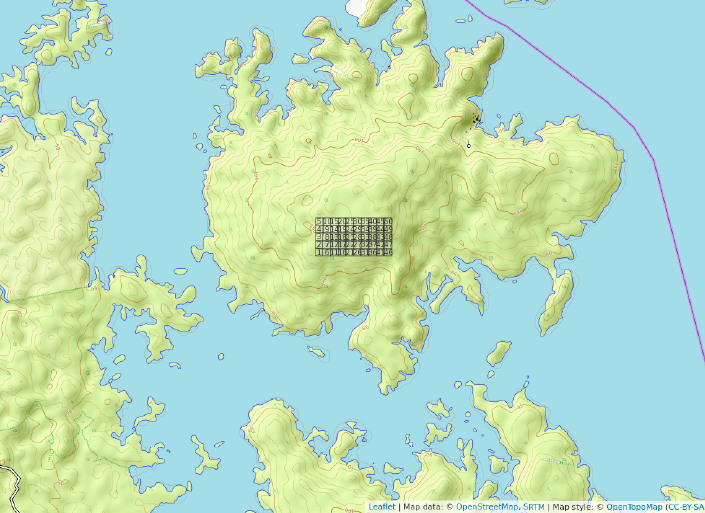
\includegraphics[width=0.50000\textwidth]{Mapa .png}
\caption{Área de estudio, parcela de 50ha, Isla Barro Colorado
\label{fig:Mapa}}
\end{figure}

\subsection{Materiales y Métodos}\label{materiales-y-muxe9todos}

La información de los cuadrantes que componen BCI fue procesada en R (R
Core Team, 2020), teniendo en cuenta la matriz ambiental y la matriz de
comunidad, los cuales contienen datos de las variables ambientales,
tales como condiciones edáficas, tipo de hábitat, topografía del lugar,
clasificación etaria del bosque, y datos demográficos y geoferenciación
espacial de todos los individuos censados. Se adaptaron scripts
reproducibles recuperados de Batlle (2020), utilizando la colección de
paquetes multifuncionales: vegan (Oksanen et al., 2019), Tidyverse
(Wickham, 2017), BiodiversityR (R. Kindt \& Coe, 2005) y indicspecies
(De Caceres \& Legendre, 2009).

Para conocer las características de los datos almacenados de la matriz
de comunidad y ambiental, se realizó un análisis exploratorio que
incluyó visualización de gráficos, tablas, mapas de los cuadrantes de
una hectárea y tablas de correlación lineal entre las dos variables de
la matriz, lo que permitió una vista común y ayudó a determinar
procedimientos más detallados a continuación.

\subsection{Medición de asociación
(ma)}\label{mediciuxf3n-de-asociaciuxf3n-ma}

Para realizar las pruebas de medición de asociación, se calculó la
distancia euclidiana entre los cuadrados considerados objetos. Para
ello, se requierió una transformación de la matriz de comunidad mediante
el método Hellinger, que incluye elevar al cuadrado la abundancia
relativa yij (cociente resultante de cada valor de abundancia entre la
suma de los sitios)(Legendre \& Gallagher, 2001). Además, se evaluó la
distancia euclidiana entre los cuadrantes en términos de ocurrencia de
especies. Se utilizó el índice de disimilitud de Jaccard de la matriz
normalizada para convertir el valor de abundancia en un valor binario
(Brocard, Gillet, \& Legendre, 2018). del mismo modo, se empleó la
métrica de Jaccard para aplicar la transposición de la matriz de la
comunidad y convertir a datos Presencia / ausencia para medir el grado
de asociación entre especies.

Para poder comparar la relación entre especies en función de su
abundancia, se utilizó estandarización \emph{ji}-cuadrado de la matriz
de comunidad transpuesta (Legendre \& Gallagher, 2001). Se examinó la
ocurrencia entre especies y su distribución en BCI por el coeficiente de
correlación entre rangos de Spearman, para medir el grado de correlación
entre las variables riqueza númerica de especies y la abundancia con las
variables ambientales geomorfológicas, y la composición química del
suelo (Brocard et al., 2018).

\subsection{Análisis de agrupamiento}\label{anuxe1lisis-de-agrupamiento}

El método jerárquico aglomerativo de asociación entre pares de
cuadrantes (según la composición de especies) bajo el estándar de enlace
completo, y el método de Ward basado en la varianza mínima, se utilizó
como método preliminar para el análisis de agrupamiento, con el fin de
probar su efectividad en lograr un grupo consistente de importancia
ecológica (Brocard et al., 2018). Luego, estos generaron dendrogramas
que posteriormente son comparados con la matriz de distancia de cuerdas
(Legendre \& Gallagher, 2001). Usando correlación cofenética entre los
dos para determinar el número ideal de grupos. Además, se utilizó
remuestreo bootstrap y boostrap multiescalar para conocer la
probabilidad de éxito de la inferencia del número de grupos y la
identidad de sus componentes (Brocard et al., 2018). Las distribuciones
se basaban en una probabilidad de 91\% o más de acierto para el método
bootstrap y de un 95\% para boostrap multiescalar.

Para conocer las especies distintas o asociadas a cada grupo, se utilizó
el valor del indicador o índice IndVal (``Conjuntos de especies y
especies indicadoras,'' 1997), basado en permutaciones aleatorias de los
sitios según la presencia de especies y la abundancia de estos. De
manera similar, el grado de asociación de una especie con una
preferencia particular por el grupo de cuadrantes considerado grupo en
estudio, expresado como el coeficiente de correlación biserial puntual
(Brocard et al., 2018). Se adoptó un enfoque similar al anterior a lo
largo de las pruebas estadísticas de la hipótesis nula, basada en las
especies presentes en los cuadrantes pertenecientes a un determinado
grupo realizado al azar. Esta prueba se hizo reordenando aleatoriamente
los valores de abundancia y comparando sus distribuciones con las
obtenidas previamente (Cáceres \& Legendre, 2009).

\subsection{Análisis de diversidad
alpha}\label{anuxe1lisis-de-diversidad-alpha}

La diversidad alpha representa la diversidad de especies a lo largo de
todas las subunidades locales relevantes, y por definición abarca dos
variables importantes: (1) la riqueza de especies, y (2) la abundancia
relativa de especies (Carmona-Galindo \& Carmona, 2013). Con el fin de
determinar la diversidad alpha se utilizaron métodos como la Entropia de
Shannon H1, que calcula el grado de desorden en la muestra, el índice de
concentración de Simpson, que calcula la probabilidad de que dos
individuos seleccionados aleatoriamente puedan ser de la misma especie.
Ademas, se empleó la serie de números de diversidad de Hill, la fórmula
de la entropía de Rengi y el índice de equidad de Pielou.

\subsection{Analisis de diversidad
beta}\label{analisis-de-diversidad-beta}

La diversidad beta, de acuerdo con (Whittaker, 1960), se define como el
diferencial entre la diversidad de un hábitat y la diversidad total de
un paisaje de hábitats. Teniendo en cuenta lo anterior, se utilizó el
metodo hellinger para determinar cuales son las especies que contribuyen
a la diversidad beta, es decir, las especies que no se encuentran
compartidas entre los cuadrantes.

\subsection{Análisis de ordenación simple (no restringida) y canónica
(restringida)}\label{anuxe1lisis-de-ordenaciuxf3n-simple-no-restringida-y-canuxf3nica-restringida}

Se aplicaron los análisis de componentes principales o PCA a los datos
de las variables ambientale para determianar la ordenacion no
restringida, donde se tomó en cuenta especificamente las variables del
suelo. y para determinar la ordenacion restringida se exploró de manera
explícita las relaciones entre una matriz de respuesta y una matriz
explicativa con los análisis de redundancia o RDA, lo cual combina la
regresión y el análisis de componentes principales (PCA), por ejemplo,
busca tendencias en la matriz de comunidad restringiéndolas a la matriz
ambiental.

\subsection{Ecología espacial}\label{ecologuxeda-espacial}

En ecología espacial se utilizó la matriz transformada de hellinger y la
matriz ambiental para crear un cuadro de vecindad y ver como se
autocorrelacionan los sitios. Se genera un correlograma para la variable
que queremos estudiar mediante la función `sp.correlogram' y para varias
variables como la abundancia de especies y las variables ambientales.
También, se utilizaron otros métodos como la prueba Mantel con matrices
de distancia para autocorrelación espacial con y sin tendencia, y el I
de Moran con una matriz de abundancia de especies transformada sin
tendencia, lo cual se aplica a variables ambientales para obtener los
datos de autocorrelación, distribución de especies y variables en los
sitios de muestreo.

\section{Resultados}\label{resultados}

Se registraron un total de 5 especies y 2 generos distribuidos en 2029
individuos en toda la parcela. La riqueza por cuadro fue de 4 especies y
la mediana de la abundancia por cuadro fue de 39 individuos. La especie
más abundante fue \emph{Pouteria reticulata}, con 1084 individuos, y la
menos abundante fue \emph{Pouteria fossicola} con 3 individuos. La tabla
\ref{tab:abun_sp} y la figura \ref{fig:abun_sp_q} resume estos
resultados. La distribución de la riqueza númerica de especies de la
familia Sapotaceae sigue un patrón homogeneo, lo cual los agregados de
riqueza máxima están distribuidos en casi todo el área (ver Figura
\ref{fig:mapa_cuadros_riq_mi_familia}). Cabe resaltar, que la
distribución de las variables ambientales PH y pendiente media siguen un
patrón relativamente similar a la distribución de la riqueza númerica de
la familia Sapotaceae.

\begin{longtable}[]{@{}lr@{}}
\caption{\label{tab:abun_sp}Abundancia por especie de la familia
Sapotaceae}\tabularnewline
\toprule
Latin & n\tabularnewline
\midrule
\endfirsthead
\toprule
Latin & n\tabularnewline
\midrule
\endhead
Pouteria reticulata & 1084\tabularnewline
Chrysophyllum argenteum & 711\tabularnewline
Chrysophyllum cainito & 171\tabularnewline
Pouteria stipitata & 60\tabularnewline
Pouteria fossicola & 3\tabularnewline
\bottomrule
\end{longtable}

\begin{figure}
\centering
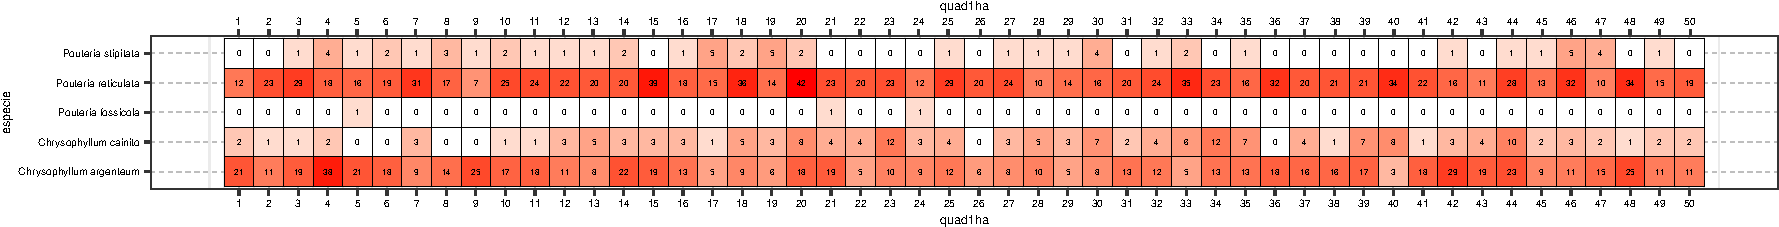
\includegraphics{manuscrito_files/figure-latex/unnamed-chunk-3-1.pdf}
\caption{\label{fig:abun_sp_q}Abundancia por especie por quadrat}
\end{figure}

\begin{figure}
\centering
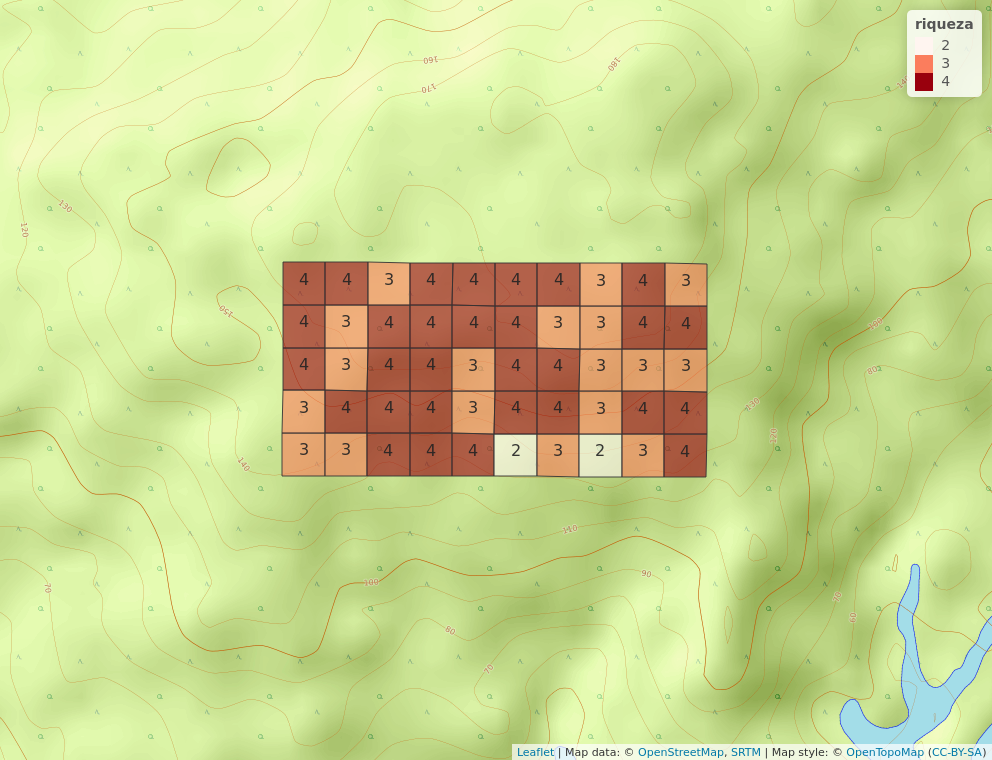
\includegraphics[width=0.50000\textwidth]{mapa_cuadros_riq_mi_familia.png}
\caption{Distribucion de la riqueza de la familia
Sapotaceae\label{fig:mapa_cuadros_riq_mi_familia}}
\end{figure}

Los valores para el coeficiente de Spearman presentados en el panel de
correlación de la figura \ref{fig:p_cor_suelo_ar}, mostraron que la
abundancia de la familia sapotaceae solo presenta correlación con la
abundacia global, mientras que la riqueza tiene correlación con la
presencia de cobre y nitrógeno en el suelo, lo que sugiere, que mientras
mas concentración de cobre y nitrógeno hay, mayor será la riqueza de
especies.

\begin{figure}
\centering
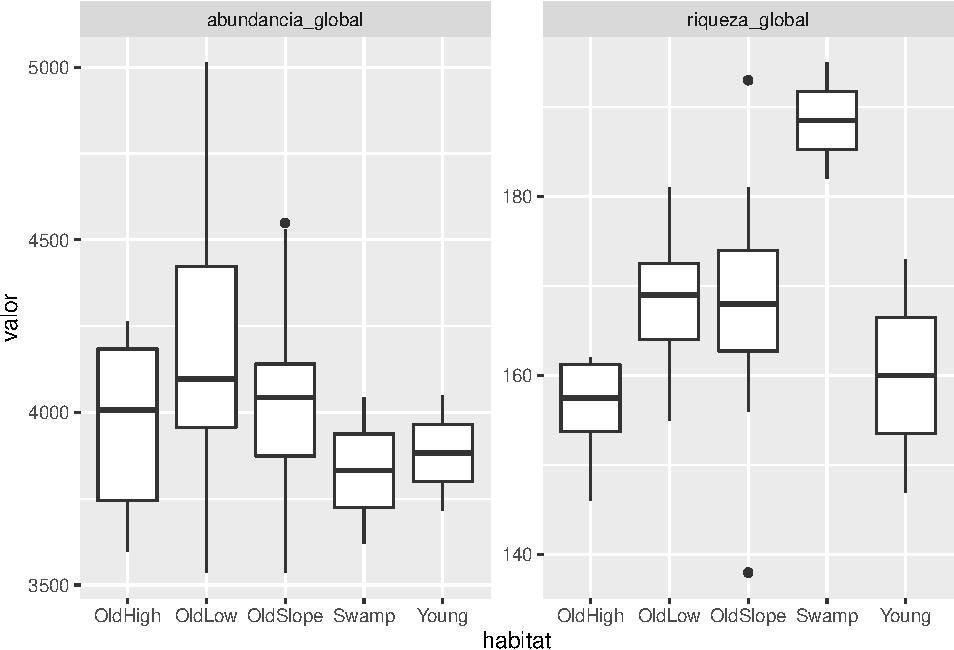
\includegraphics{manuscrito_files/figure-latex/unnamed-chunk-4-1.pdf}
\caption{\label{fig:p_cor_suelo_ar}correlacion de las variables del
suelo}
\end{figure}

El índice de similaridad de Jaccard muestra que el sitio 1 y 2 comparten
un 100\% de sus especies, por lo que ambos sitios comparten 3 especies y
no tienen especies exclusivas (ver figura
\ref{fig:similaridad_jaccard}). Las variables geomorfológicas presentan
asociación con la abundancia y riqueza, lo cual la figura
\ref{fig:matriz_correlacion_geomorf_abun_riq_spearman} muestra que hay
mucha similaridad entre estas variables. Las pruebas de correlación
entre los grupos 1 y 2 formulados por upgma resultaron significativas
respecto a la variable fósforo. Por otro lado, el contenido de cobre y
la abundancia global promedio, es decir, la media correspondiente a
todas las plantas en BCI, son significativamente diferentes entre los
sitios de ambos grupos, para un nivel de significancia de a = 0.1(ver
figura \ref{fig:grupos_upgma}).

El grupo 1 generado por enlace upgm esta conformado por 5 cuadrante y el
grupo 2 por 46 cuadrantes (ver figura \ref{fig:mapa_upgma_k2}). El grupo
2 contiene los sitios con tendencia a presentar valores altos de zinc y
contenido de cobre. Es probable que las especies indicadoras del grupo
con un mayor contenido de cobre estén mostrando preferencia por estas
condiciones ambientales. No obstante, la mayoría de componentes del
suelo en BCI tienen valores bastante homogéneos, y más bien se presentan
pequeños gradientes entre los cuadrantes, lo cual evita que este tipo de
acercamiento sea concluyente. La especie \emph{Chrysophyllum argenteum}
fué la que obtuvo un valor alto de confianza al examinar su potencial
como especies indicadoras del grupo 1. Para el caso del grupo 2, la
especie indicadora fué \emph{Pouteria reticulata}.

\begin{figure}
\centering
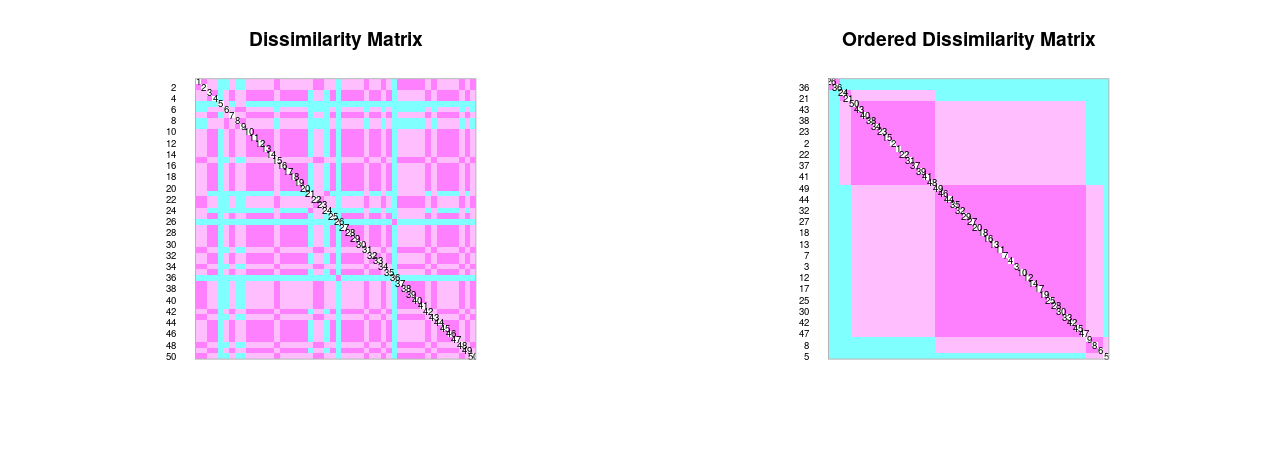
\includegraphics[width=1.00000\textwidth]{Similaridad.png}
\caption{Similaridad de Jaccard (color fucsia (magenta, rosa) significa
``corta distancia=muy similares'', y cian (celeste) significa ``gran
distancia=poco similares'')\label{fig:similaridad_jaccard}}
\end{figure}

\begin{figure}
\centering
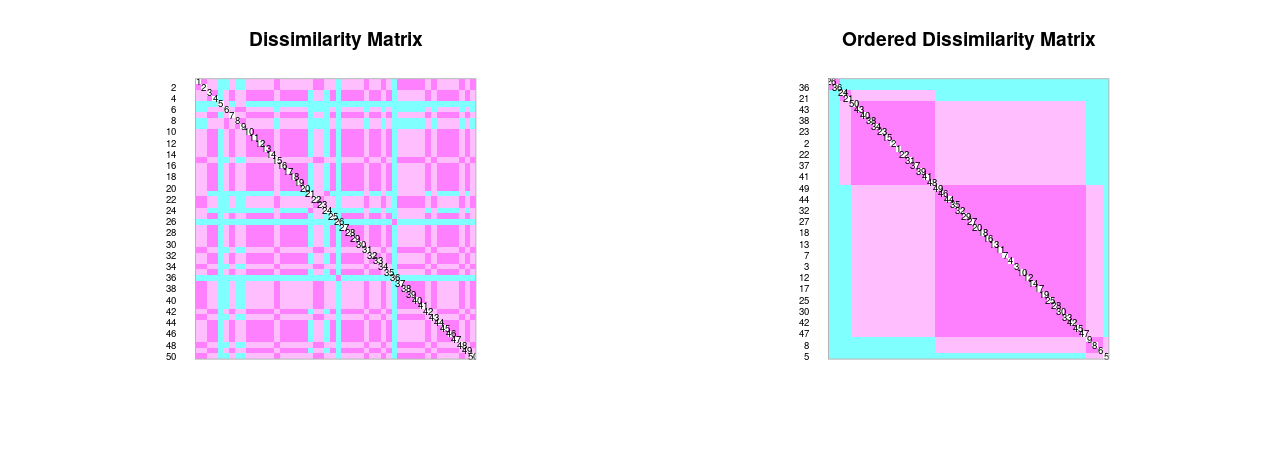
\includegraphics[width=1.00000\textwidth]{Similaridad.png}
\caption{Panel de correlacion de Spearman entre los datos de la
comunidad y las variables geomorfologicas (color fucsia (magenta, rosa)
significa ``corta distancia=muy similares'', y cian (celeste) significa
``gran distancia=poco
similares'')\label{fig:matriz_correlacion_geomorf_abun_riq_spearman}}
\end{figure}

\begin{figure}
\centering
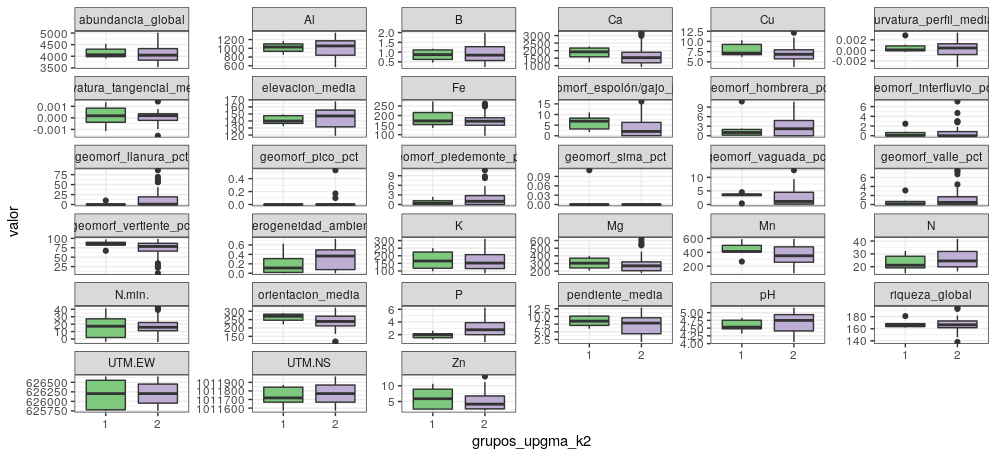
\includegraphics[width=1.00000\textwidth]{actualizacion2_grupos_upgma.png}
\caption{Diagramas de caja de las variables que tuvieron un efecto,
segun las pruebas de igualdad de medias\label{fig:grupos_upgma}}
\end{figure}

\begin{figure}
\centering
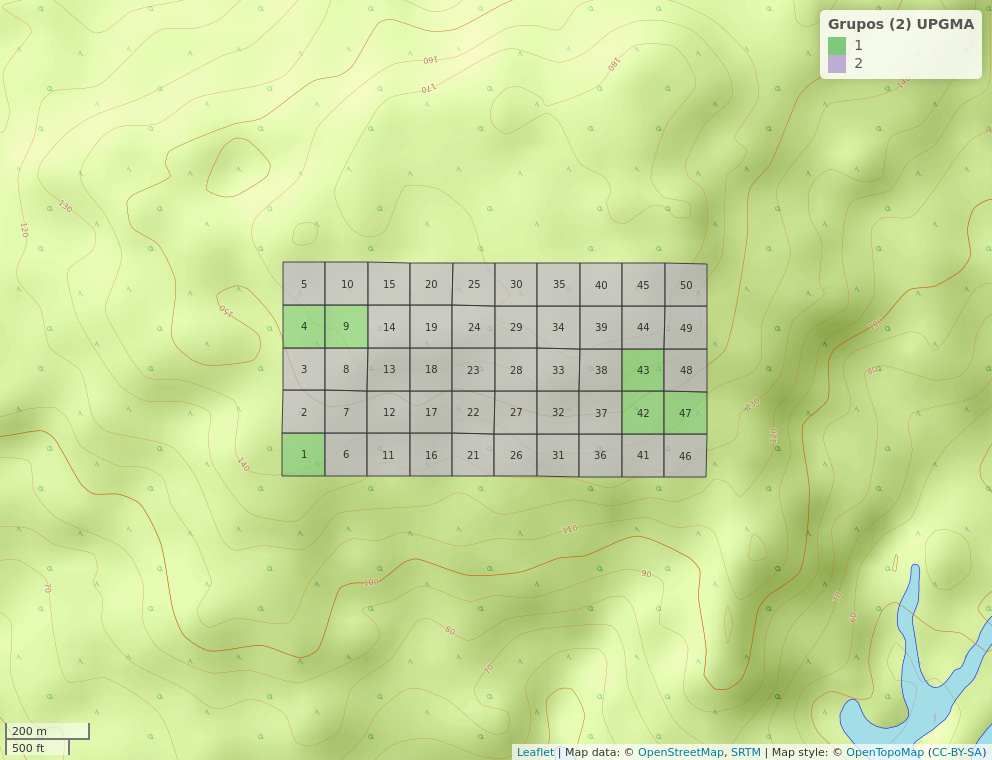
\includegraphics[width=0.50000\textwidth]{mapa_upgma_k2.png}
\caption{Mapa en el que se presenta la distribucion de sitios en los
grupos formulados por enlace upgma\label{fig:mapa_upgma_k2}}
\end{figure}

La riqueza de la familia Sapotaceae aumenta en función del contenido de
hidrógeno, nitrógeno y cobre. Ademas, aunmenta con la equidad. Cabe
destacar, que algunos sitios de BCI tienen valores altos de equidad (ver
figura \ref{fig:grafico_niveles_equidad}). La Curva de rarefaccion de
los sitios, muestra como va aumentando la cantidad de individuos y de
especies de los cuadrantes (ver figura \ref{fig:Curva_rarefaccion}),
donde la mayor concentración de individuos está entre los 20 a 50
individuos y la abundancia maxima es de 70 individuos. Los valores de
los indices de diversidad alfa fueron: Species Richness 0.217, Shannon
diversity 0.045 y Simpson diversity 0.038.

\begin{figure}
\centering
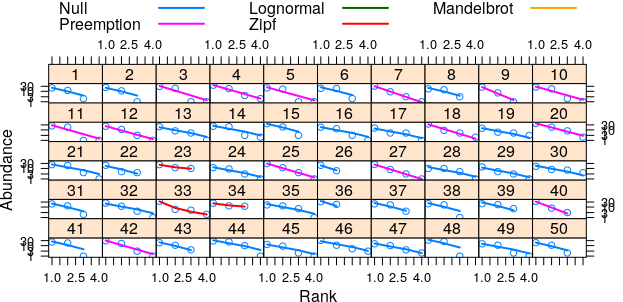
\includegraphics{grafico_niveles_equidad.png}
\caption{Grafico dque presenta los valores de equidad por sitos
\label{fig:grafico_niveles_equidad}}
\end{figure}

\begin{figure}
\centering
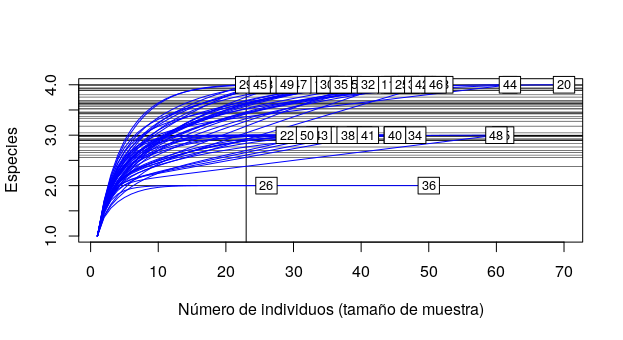
\includegraphics{Curva_rarefaccion.png}
\caption{Curva de rarefaccion de los sitios
\label{fig:Curva_rarefaccion}}
\end{figure}

Las especies que contribuyen de manera significativa a la diversidad
beta fueron: \emph{Chrysophyllum argenteum} (0.2504234),
\emph{Chrysophyllum cainito} (0.3147978) y \emph{Pouteria stipitata}
(0.2658814), de las cuales la que mas contribuyó a la diversidad beta
fué \emph{Chrysophyllum cainito}. No obstante, los sitios que
contribuyen a la diversidad beta son los cuadrantes 9 y 40, lo cual
presentan contribución a la diversidad beta por la incidencia de algunas
variables ambientales.

El grafico \ref{fig:env_suelo_pca} incluye el comportamiento de los
componentes principales de la varianza en las variables suelo y
geomorfologia en BCI, predecido por el modelo de barra quebrada,
representado por la línea roja formando la curva (La escala denominada
``Inertia'' representa la suma de los cuadrados de toda la varianza). En
el diagrama rotulado como escalamiento 1 de la figura
\ref{fig:Biplot_PCA_escalamiento}, se observan tres grupos de cuadrantes
diferenciados entre sí. Un grupo de sitios con un alto grado de acidez y
contenido en aluminio, otro grupo caracterizado por la presencia de
elementos metálicos, y un tercero, con una cantidad de fósforo,
nitrógeno y valor de pH mayor. Las variables nitrógeno, fósforo y pH
aportan la mayor parte de la varianza explicada. La relación entre las
variables se encuentra debidamente representada en el recuadro del
escalamiento 2, por medio de los ángulos que forman sus vectores (ver
figura \ref{fig:Biplot_PCA_escalamiento}). Los resultados del PCA de los
datos de la matriz de comunidad se encuentran resumidos en los diagramas
de la figura \ref{fig:PCA_comunidad}. El escalamiento 1, muestra muchos
de los cuadrantes dispuestos alrededor del origen formado por los ejes,
lo que indica una contribución a la varianza relativamente equitativa
por parte de las especies.

\begin{figure}
\centering
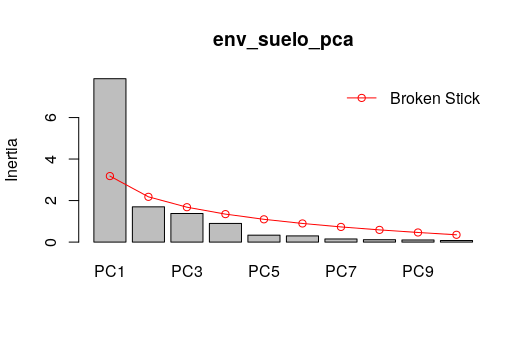
\includegraphics{env_suelo_pca.png}
\caption{grafico de los componentes principales de la varianza en las
variables suelo y geomorfologia en BCI \label{fig:env_suelo_pca}}
\end{figure}

\begin{figure}
\centering
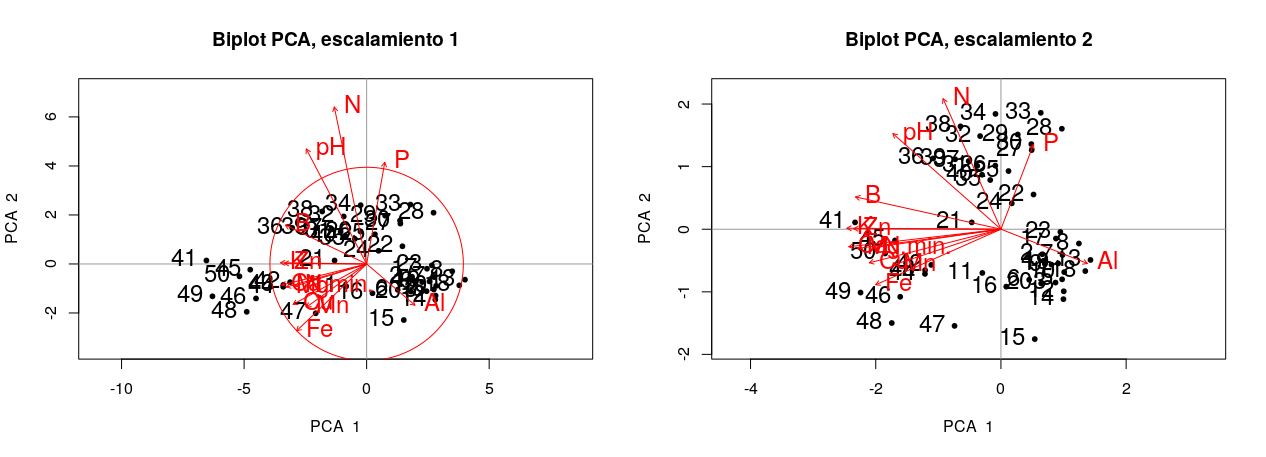
\includegraphics[width=1.00000\textwidth]{Biplot_PCA_escalamiento_actualizado.png}
\caption{Biplots generados en el PCA de las viariables de suelo
\label{fig:Biplot_PCA_escalamiento}}
\end{figure}

\begin{figure}
\centering
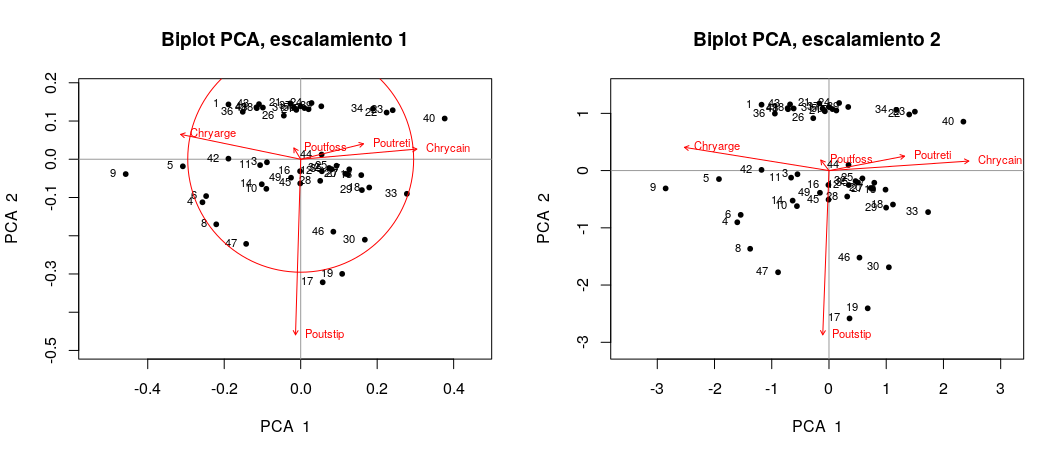
\includegraphics[width=1.00000\textwidth]{PCA_comunidad_actualizado.png}
\caption{Biplots generados en el PCA de las viariables de suelo
\label{fig:PCA_comunidad}}
\end{figure}

El escalamiento 2 de la figura \ref{fig:Analisis_de_correspondencia} en
el análisis de correspondencia mostró que las especies \emph{Pouteria
reticulata}, \emph{Chrysophyllum argenteum} y \emph{Chrysophyllum
cainito} se encuentran asociadas. Las especies restantes tienen una
abundancia reducida, y en consecuencia, aparecen cercanas a los pocos
cuadrantes en los que se encuentran representadas. La disparidad en la
incidencia de las especies se refleja en su disposición en el diagrama.
Sin embargo, estos resultados no coinciden del todo con los arrojados
por el PCA de la matriz de distancias.

Los primero ordenes de \emph{Chrysophyllum argenteum} y
\emph{Chrysophyllum cainito} presentan valores de autocorrelación alta o
positiva, mientras que los ordenes de las demas especies presentan
mayormente valores de autocorrelación negativa (Ver figura
\ref{fig:Abundancia_matriz}).

\begin{figure}
\centering
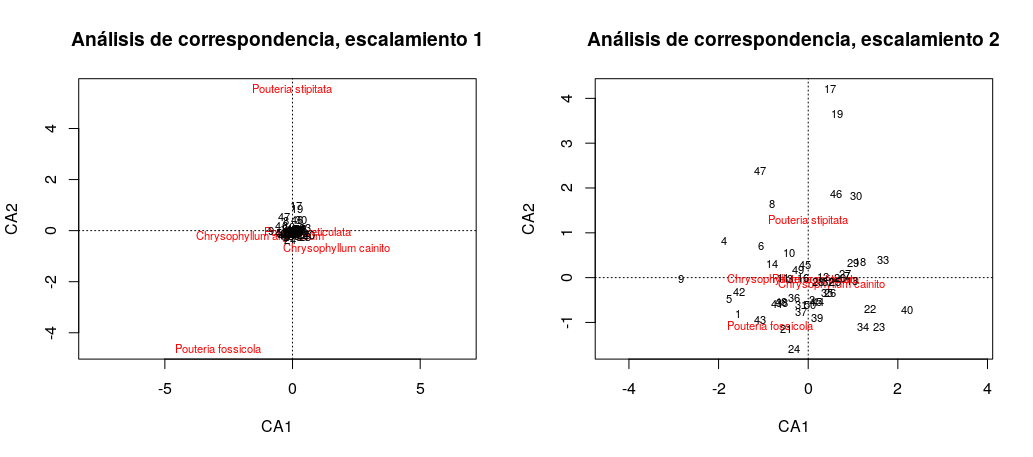
\includegraphics[width=1.00000\textwidth]{analisis_de_correspondencia_actualizado.png}
\caption{Biplot del analisis de correspondencia de los datos de
abundancia de las especies de Sapotaceae
\label{fig:Analisis_de_correspondencia}}
\end{figure}

\begin{figure}
\centering
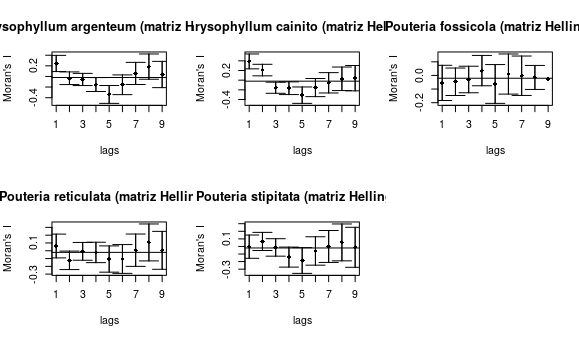
\includegraphics[width=1.00000\textwidth]{Abundancia_matriz.png}
\caption{Autocorrelación espacial de las especies
\label{fig:Abundancia_matriz}}
\end{figure}

\section{Discusión}\label{discusiuxf3n}

Estudios de la familia Sapotaceae también reportan que \emph{Pouteria}
es un genero que parece siempre presentar una cantidad significativa de
individuos (Martínez-Sovero et al. (2021)). La riqueza de la familia
Sapotaceae aumenta en función del contenido de hidrógeno, nitrógeno y
cobre, los cuales son algunos de los nutrientes que más se correlacionan
con la diversidad de especies de plantas en el neotrópico (Doblado
Amador (2011)). Ademas, la riqueza aunmenta con la equidad, por lo que
casi todos los sitios de BCI tienen valores altos de equidad, debido a
que las especies estan distribuidas en casi todos los cuadrantes.

Los valores de los indices de diversidad alfa fueron: Species Richness
0.217, Shannon diversity 0.045 y Simpson diversity 0.038lo, estos
valores sugieren que la familia Sapotaceae no presenta mucha diversidad
en BCI. Se estima que la riqueza seguiría constante o no aumentaria
significativamente aunque se hiciera mayor esfuerzo de muestreo (ver
figura\ref{fig:acumulacion_especies_individuos}).

\begin{figure}
\centering
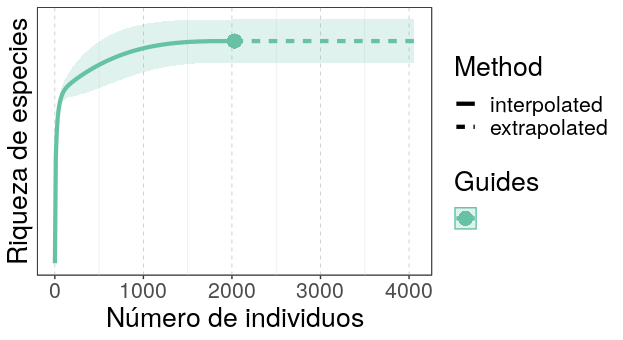
\includegraphics{acumulacion_especies_individuos.png}
\caption{Grafico de acumulacion de especies en funcion de numeros de
individuos \label{fig:acumulacion_especies_individuos}}
\end{figure}

Las especies que contribuyen de manera significativa a la diversidad
beta fueron: \emph{Chrysophyllum argenteum}, \emph{Chrysophyllum
cainito} y \emph{Pouteria stipitata}, las cuales fueron las que
obtuvieron valores intermedios de individuos. No obstante, los sitios
que contribuyen a la diversidad beta son los cuadrantes 9 y 40, lo cual
presentan contribución a la diversidad beta por la incidencia de algunas
variables ambientales, tales como el ph, aluminio, boro,
manganeso\ldots{} Las especies \emph{Pouteria reticulata},
\emph{Chrysophyllum argenteum} y \emph{Chrysophyllum cainito} se
encuentran asociadas, debido a que tienen los valores mas altos de
abundancia dentro de la comunidad (1084, 711 y 171 individuos,
respectivamente).

Los primero ordenes de \emph{Chrysophyllum argenteum} y
\emph{Chrysophyllum cainito} presentan valores de autocorrelación
positiva, mientras que los ordenes de las demás especies presentan
mayormente valores de autocorrelación negativa, teniendo en cuenta que
el orden 5 de todas las especies presenta autocorrelacion negativa, lo
que sugiere que el orden 5 de las especies está autocorrelacionado
espacialmente negativo.

\section{Agradecimientos}\label{agradecimientos}

Agradezco al maestro José Ramón Martinez, por su motivación y ayuda en
todos los aspectos para que este trabajo salga bien.

\section{Información de soporte}\label{informaciuxf3n-de-soporte}

\ldots

\section{\texorpdfstring{\emph{Script}
reproducible}{Script reproducible}}\label{script-reproducible}

\section*{Referencias}\label{referencias}
\addcontentsline{toc}{section}{Referencias}

\hypertarget{refs}{}
\hypertarget{ref-jose_ramon_martinez_batlle_2020_4402362}{}
Batlle, J. R. M. (2020). biogeografia-master/scripts-de-analisis-BCI:
Long coding sessions (Version v0.0.0.9000).
\url{https://doi.org/10.5281/zenodo.4402362}

\hypertarget{ref-brocard2011numerical}{}
Brocard, D., Gillet, F., \& Legendre, P. (2018). Numerical ecology with
r. \emph{Springer Nature}, \emph{Second Edition}, 52--66. Retrieved from
\url{https://doi.org/10.1007/978-3-319-71404-2}

\hypertarget{ref-campos2017analisis}{}
Campos-Pineda, E. G., Moreno, J., \& Mendieta, J. (2017). Análisis
florístico de la vegetación arbórea de una parcela de bosque en el
parque natural metropolitano, provincia de panamá. \emph{Scientia},
\emph{27}(1), 7--24.

\hypertarget{ref-carmona2013diversidad}{}
Carmona-Galindo, V. D., \& Carmona, T. V. (2013). La diversidad de los
análisis de diversidad la diversidad de los analisis de diversidad
{[}the diversity of diversity analyses{]}. \emph{Bioma}.

\hypertarget{ref-caceres2009associations}{}
Cáceres, M. D., \& Legendre, P. (2009). Associations between species and
groups of sites: Indices and statistical inference. \emph{Ecology},
\emph{90}(12), 3566--3574.

\hypertarget{ref-condit2012thirty}{}
Condit, R. A. y H., Richard y Chisholm. (2012). Treinta años de censo
forestal en barro colorado y la importancia de la inmigración para
mantener la diversidad. \emph{PloS One}, \emph{7}(11), e49826.

\hypertarget{ref-condit2017demographic}{}
Condit, R. y L., Richard y Pérez. (2017). Tendencias demográficas y
clima durante 35 años en la parcela de 50 ha de barro colorado.
\emph{Forest Ecosystems}, \emph{4}(1), 1--13.

\hypertarget{ref-condit2002beta}{}
Condit, R., Pitman, N., Leigh, E. G., Chave, J., Terborgh, J., Foster,
R. B., \ldots{} others. (2002). Beta-diversity in tropical forest trees.
\emph{Science}, \emph{295}(5555), 666--669.

\hypertarget{ref-dufrene1997species}{}
Conjuntos de especies y especies indicadoras: La necesidad de un enfoque
asimétrico flexible. (1997). \emph{Monografías Ecológicas},
\emph{67}(3), 345--366.

\hypertarget{ref-indicspecies}{}
De Caceres, M., \& Legendre, P. (2009). Associations between species and
groups of sites: Indices and statistical inference. In \emph{Ecology}.
Retrieved from \url{http://sites.google.com/site/miqueldecaceres/}

\hypertarget{ref-doblado2011identificacion}{}
Doblado Amador, L. S. (2011). Identificación y caracterización de tipos
de bosque y su relación con variables ambientales, en un paisaje
fragmentado al norte de honduras. \emph{Proyecto Finnfor I Y Finnfor
II-CATIE}.

\hypertarget{ref-horvat2010spatially}{}
Horvát, S., Derzsi, A., Néda, Z., \& Balog, A. (2010). A spatially
explicit model for tropical tree diversity patterns. \emph{Journal of
Theoretical Biology}, \emph{265}(4), 517--523.

\hypertarget{ref-leigh1990barro}{}
Isla barro colorado y biología tropical. (1990). \emph{Cuatro Bosques
Neotropicales}, 28--47.

\hypertarget{ref-diversityanalysis}{}
Kindt, R., \& Coe, R. (2005). \emph{Tree diversity analysis. a manual
and software for common statistical methods for ecological and
biodiversity studies}. Retrieved from
\url{http://www.worldagroforestry.org/output/tree-diversity-analysis}

\hypertarget{ref-legendre2001ecologically}{}
Legendre, P., \& Gallagher, E. D. (2001). Ecologically meaningful
transformations for ordination of species data. \emph{Oecologia},
\emph{129}(2), 271--280.

\hypertarget{ref-martinez2020importancia}{}
Martínez-Sovero, G., Iglesias-Osores, S., \& Villena-Velásquez, J. J.
(2020). Importancia de la familia sapotaceae en madre de dios, perú.
\emph{Manglar}, \emph{17}(4), 287.

\hypertarget{ref-martinez2021diversidad}{}
Martínez-Sovero, G., Iglesias-Osores, S., Muñoz-Chavarry, P.,
Seminario-Cunya, A., Alva-Mendoza, D., \& Villena-Velásquez, J. (2021).
Diversidad y estructura de sapotaceae en bosques amazónicos de madre de
dios, perú. \emph{Ciencia Amazónica (Iquitos)}, \emph{9}(1), 59--72.

\hypertarget{ref-vegan}{}
Oksanen, J., Blanchet, F. G., Friendly, M., Kindt, R., Legendre, P.,
McGlinn, D., \ldots{} Wagner, H. (2019). \emph{Vegan: Community ecology
package}. Retrieved from \url{https://CRAN.R-project.org/package=vegan}

\hypertarget{ref-perez2005metodologia}{}
Pérez, R., Aguilar, S., Condit, R., Foster, R., Hubbell, S., \& Lao, S.
(2005). Metodologia empleada en los censos de la parcela de 50 hectareas
de la isla de barro colorado, panamá. \emph{Centro de Ciencias
Forestales Del Tropico (CTFS) Y Instituto Smithsonian de Investigaciones
Tropicales (STRI)}, 1--24.

\hypertarget{ref-Restudio}{}
R Core Team. (2020). \emph{R: A language and environment for statistical
computing}. Retrieved from \url{https://www.R-project.org/}

\hypertarget{ref-rodriguez2020scolytinae}{}
Rodríguez-Flores, W., \& Barrios, H. (2020). Scolytinae y platypodinae
(coleoptera: Curculionidae) de la isla barro colorado, panamá.
\emph{Scientia}, \emph{30}(1), 15--52.

\hypertarget{ref-smedmark2007boreotropical}{}
Smedmark, A. A., Jenny EE y Anderberg. (2007). La migración
boreotropical explica la hibridación entre linajes geográficamente
distantes en el clado pantropical sideroxyleae (sapotaceae).
\emph{American Journal of Botany}, \emph{94}(9), 1491--1505.

\hypertarget{ref-wan2020importancia}{}
Wan, D. (2020). IMPORTANCIA de los bosques y estado de los bosques en
guatemala. \emph{Revista Ingeniería Y Ciencia}, \emph{2}(12).

\hypertarget{ref-whittaker1960vegetation}{}
Whittaker, R. H. (1960). Vegetation of the siskiyou mountains, oregon
and california. \emph{Ecological Monographs}, \emph{30}(3), 279--338.

\hypertarget{ref-tidyverse}{}
Wickham, H. (2017). \emph{Tidyverse: Easily install and load the
'tidyverse'}. Retrieved from
\url{https://CRAN.R-project.org/package=tidyverse}

\hypertarget{ref-windsorestructura}{}
Windsor, D., FOSTER, R., BROKAW, N., Leigh, E., Rand, A., \& others.
(1990). \emph{Estructura e historia de la vegetación de la isla barro
coloradoecología de un bosque tropical: Ciclos estacionales y cambios a
largo plazo} (pp. 113--127).




\newpage
\singlespacing 
\end{document}
